\chapter{Estabilidad Estructural}

En esta unidad temática se consideran nuevas referencias, dado que se debe introducir un concepto fundamentalmente diferente al resto de las unidades temáticas. %
%
La hipótesis fundamental modificada: es que el equilibrio deja de realizarse en la configuración de referencia para realizarlo en una configuración deformada (bajo hipótesis de pequeños giros), permitiendo modelar el fenómeno de \textit{inestabilidad estructural}. %
%
Las principales referencias utilizadas son \citep{yoo2011,Bazzano2017}. 

\section{Conceptos fundamentales} 

En esta sección se presentan coneptos y herramientas fundamentales para poder abordar el estudio de las ecuaciones que gobiernan el fenómeno de estabilidad estructural.

\subsection{Breve revisión histórica y motivación}

El inicio del estudio de la estabilidad elástica de elementos estructurales se remonta al trabajo de Leonard Euler, quien en 1757 presentó un resultado que sigue siendo hoy en día central para el análisis y diseño de columnas esbeltas. %
%
Euler determinó que, para una columna con proporcionalidad entre momento flector y curvatura, existe un valor de compresión crítica a partir de la cual, la columna pierde la estabilidad. %
%
El lector interesado podrá ver más detalles del trabajo pionero de Euler en \citep{Timoshenko1953}.

El fenómeno de la inestabilidad elástica se tornó un tema cada vez más relevante con la adopción del hierro (y posteriormente el acero) como material de construcción. %
%
Se debe recordar que el primer puente de hierro se construyó en Coalbrookdale, Inglaterra en 1781 y el primer puente de celosía de acero se construyó sobre el río Mississipi, EEUU en 1868.  Estos materiales permitieron la construcción de estructuras con componentes cada vez más esbeltos. 

En este contexto, hubo un número considerable de colapsos debido a fallos por inestabilidad elástica. %
%
Tanto la clara representación del fenómeno de inestabilidad, como sus trágicas consecuencias, hacen de algunos fallos, casos de estudio típicos de interés para estudiantes de Ingeniería. %
%
Uno de ellos se dio en 1907 en la construcción del puente sobre el río Quebec en Canadá analizado en \citep{Brady2014}. %
%
La estructura del puente contaba con ménsulas balanceadas y un vano libre de $549$ metros. %

Una serie de errores, omisiones y malas prácticas llevaron al colapso del puente. En última instancia, el colapso se debió a una falla por inestabilidad de un barra sometida a gran compresión, resultando en la muerte de $75$ operarios. Se recomienda leer el artículo referenciado para conocer más detalles de este caso.

En tiempos más recientes, una serie de colapsos se dieron en un corto plazo de tiempo en una tipología estructural de puente que se estaba popularizando en ese momento. %
%
Los puentes con sección cajón de acero de Milford Haven de 1970 en Gales, Koblenz de 1971 en Alemania y West Gate de 1970 en Australia, son algunos de los casos en dicha serie de colapsos. %
%
En todos ellos, la inestabilidad de las placas de acero, que conforman los cajones, fue un factor determinante en los colapsos. %
%
Consultar el artículo de \cite{Firth2010}\footnote{Disponible en \href{https://www.istructe.org/webtest/files/48/488ca532-a956-4929-9f50-aee0d5317afc.pdf}{istructe.org/webtest/files/48/488ca532-a956-4929-9f50-aee0d5317afc.pdf}, últ. acceso 15/Nov/2020} para conocer la historia de dicha tipología, así como la serie de colapsos en la década de los 70.

Estos colapsos fueron el disparador de un gran esfuerzo de investigación en estructuras con el objetivo de generar reglas de diseño para evitar nuevos accidentes en esta clase de estructuras. %
%
En Inglaterra, dicho impulso resultó en la serie de reglas de diseño conocidas como IDWR, que luego pasarían a formar parte de BS 5400-3, la antigua norma británica para diseño de puentes de acero, hoy reemplazada por el Eurocódigo EN 1993. %
%
Dicha investigación avanzó enormemente el entendimiento de cómo se comportan los cajones de acero, en particular la estabilidad de las chapas rigidizadas que los componen. El lector interesado puede leer el reporte de la comisión investigadora del colapso de West Gate\footnote{Disponible en \href{http://www.parliament.vic.gov.au/papers/govpub/VPARL1971-72No2.pdf}{parliament.vic.gov.au/papers/govpub/VPARL1971-72No2.pdf}, ult. acceso 15/Nov/2020}, en el cual se puede apreciar la magnitud y complejidad de la estructura que colapsó. 

Las normas modernas exigen, o permiten, que los problemas comunes de inestabilidad sean considerados mediante reglas relativamente sencillas. Todos los materiales incluyen reglas en sus respectivas normas para la evaluación de la estabilidad estructural, tanto a nivel de componentes así como a nivel global de la estructura. %
Sin embargo, el diseño de estructuras de acero es el que hace mayor hincapié en este tema, dado que en general dichas estructuras se forman a partir de un gran número de componentes esbeltos. 

A modo de ejemplo, se refiere a la sección E3 de la norma AISC 360-16 o sección 6.3.1 de la norma EN 1993-1-1 para ver el tratamiento de resistencia axial de columnas esbeltas de acero que fallan por inestabilidad. %
%
El lector encontrará que las normas hacen referencia a $F_e$ (AISC 360-16) y $N_{cr}$ (EN 1993-1-1) que son esencialmente la carga crítica que Euler descubrió en 1757.

Las normas técnicas exigen también la evaluación de la estabilidad global de la estructura. El capítulo C de la norma AISC 360-16 trata sobre este tema, mientras que la norma EN 1992-1-1 lo hace en el Anexo H. %
%
En pocas palabras, se requiere que el profesional evalúe la estabilidad de la estructura en su conjunto y que determine los efectos que puedan surgir de la esbeltez global de la estructura. Estas evaluaciones son parte básica del trabajo del profesional que diseña una estructura.

Finalmente, como motivación se muestran diagramas de deformadas de dos modelos computacionales con inestabilidad. En la Figura~\ref{fig:PandeoChapa} se muestra un modelo de una chapa sometida a cargas de compresión meridional, mientras que en la Figura~\ref{fig:PandeoViga} se observa una viga sometida a cargas verticales mostrando pandeo lateral. 
%
\begin{figure}[htb]
	\centering
	\subfloat[Pandeo de Chapa a compresión]{
		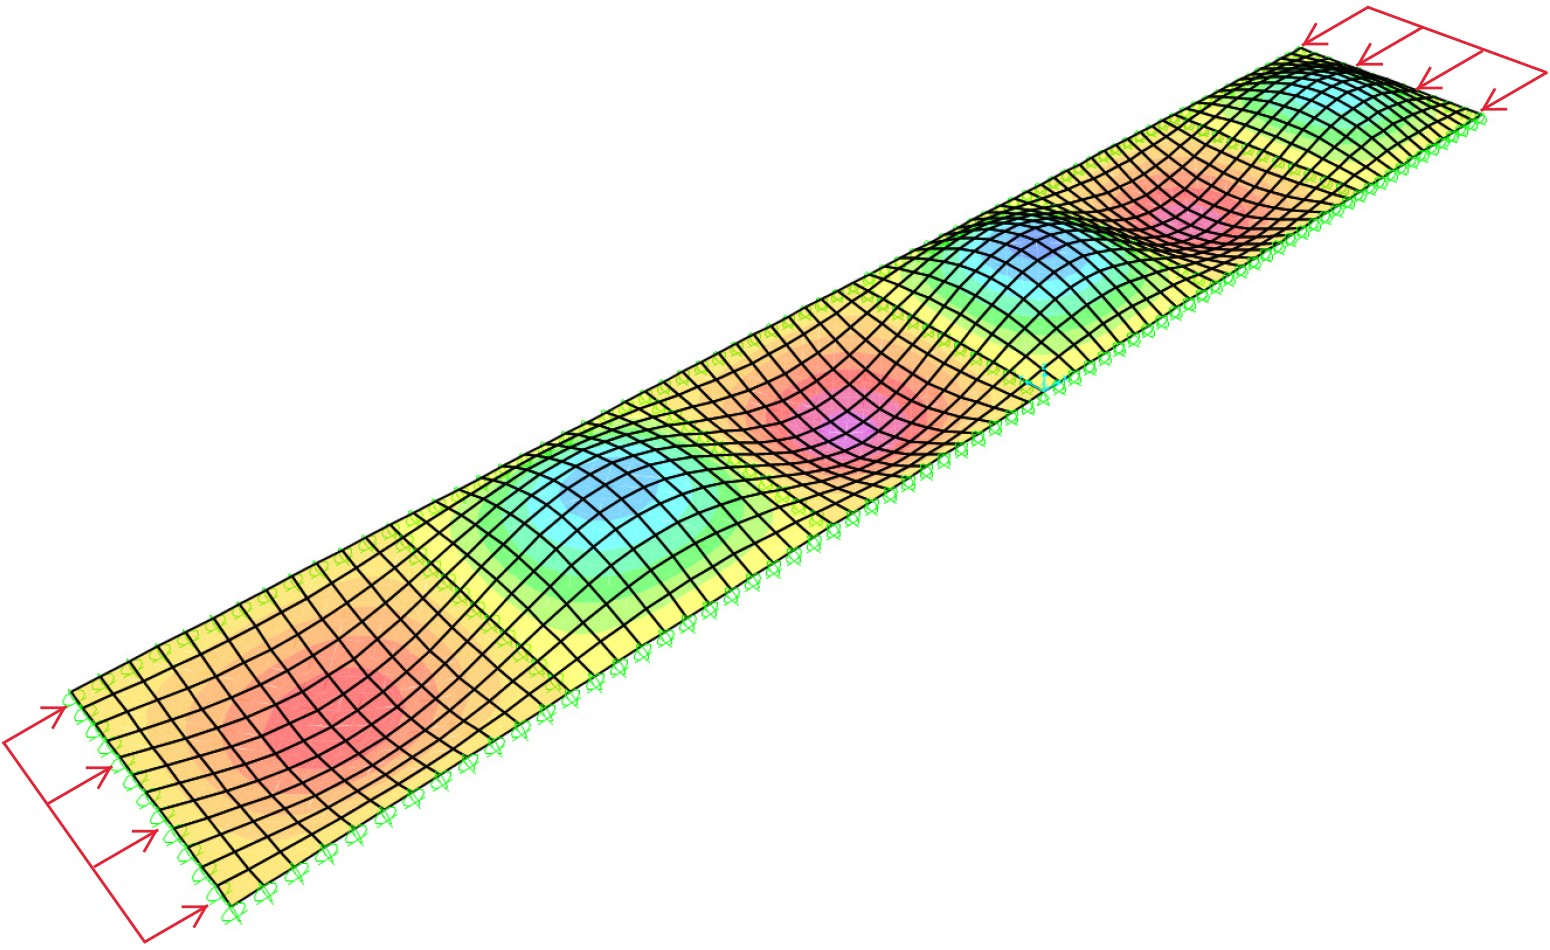
\includegraphics[width=0.42\textwidth]{PandeoChapa}
		\label{fig:PandeoChapa}}
	\hfill
	\subfloat[Pandeo lateral de viga por flexión]{
		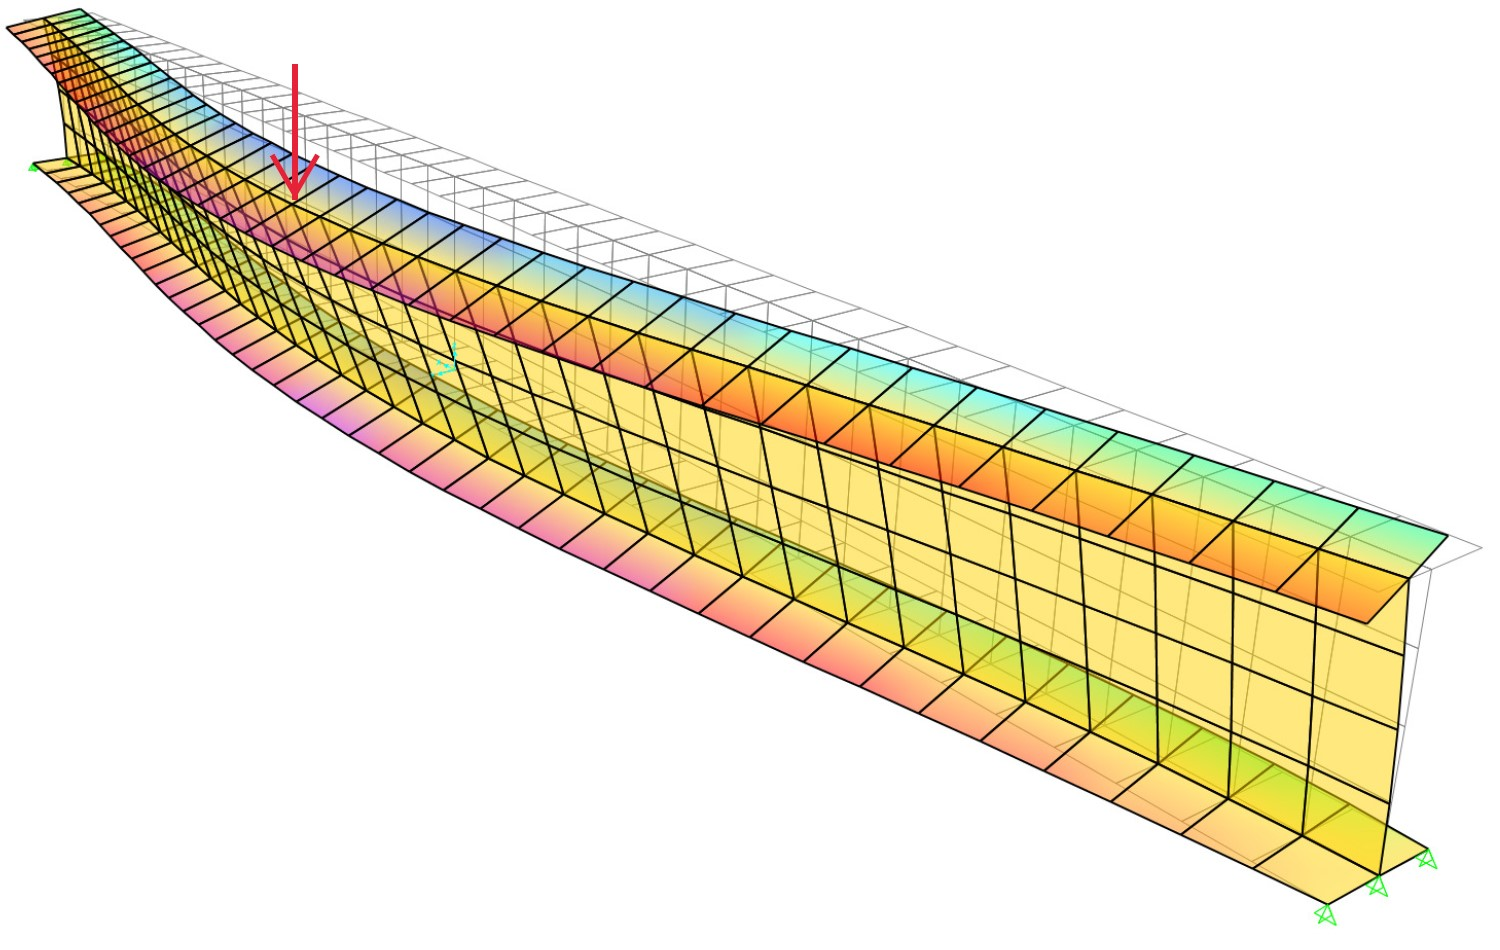
\includegraphics[width=0.42\textwidth]{PandeoViga}
		\label{fig:PandeoViga}}
	\caption{Ejemplos de inestibilidades en elementos estructurales.}
	\label{fig:PandeoContinuo}
\end{figure}

Ambos elementos y cargas estructurales están presenten en puentes del tipo de los citados en la revisión histórica. Se cuenta entonces con la motivación de entender los modelos matemáticos que permiten predecir y evitar este tipo de fenómenos y las consecuentes fallas.

% -----------------------------------------------------------
\subsection{Principio de Mínima Energía Potencial Total}


\subsubsection{Equilibrio y estabilidad} 

En las unidades temáticas anteriores, se han definido y aplicado las condiciones que la configuración deformada de una estructura debe satisfacer para ser solución del problema de Elasticidad Lineal (equilibrio, compatibilidad de deformaciones y relación tensión deformación lineal). En particular, se aplicó la formulación basada en el Principio de Mínima Energía Potencial Total, como solución del siguiente problema de minimización:

\begin{equation}\label{eqn:minPi}
\bfu = \arg\min_{\bfu\in\mcU} \quad  \Pi(\bfu)
\end{equation}

En esta Unidad Temática se introduce del concepto de \textit{Estabilidad} dado por la siguiente definición.

\cajaconcepto{Definición: Estabilidad estructural}
{Dada una estructura sometida a cargas externas dadas y dada una \textit{configuración deformada} en equilibrio con dichas cargas, se dice que la configuración es \textit{estable} si, dicha configuración es mantenida luego de aplicar una perturbación arbitraria pequeña a la estructura.}

La condición de mínima energía potencial total no solo garantiza el equilibrio de las estructuras, sino que también implica la estabilidad de las mismas.

\subsubsection{Caso lineal}

Para el modelo estructural lineal (i.e. equilibrio en la configuración de referencia, pequeños desplazamientos y material elástico lineal) se vio que la energía potencial total de la estructura está dada por la expresión general:
%
\begin{equation}\label{eqn:pilineal}
\Pi(\bfu)= \frac{1}{2} \bfu \cdot \bfK \bfu - \bfF_G \cdot \bfu
\end{equation}
%
donde $\bfF_G$ es el vector de fuerzas generalizadas y $\bfK$ la matriz de rigidez. %
Se puede verificar que para estructuras con condiciones de apoyo suficientes y que no tengan mecanismos internos o externos, se tiene una matriz de rigidez definida positiva. Esto es equivalente a:
\begin{equation}\label{eqn:Kdefpos}
\bfu \cdot \bfK \bfu > 0 \quad \forall \bfu\neq 0 \in \mcU.
\end{equation}

Calculando la hessiana de $\Pi$ y usando la Ecuación~\ref{eqn:Kdefpos} se muestra que en caso de encontrar una configuración de equilibrio que minimice $\Pi$, se tiene automáticamente que esta es estable, ya que el mínimo es estricto, y único.  

Se concluye entonces que \textbf{los modelos estructurales lineales}, \textbf{no permiten modelar} la \textbf{inestabilidad} elástica de una estructura. %

Para poder estudiar el fenómeno de inestabilidad, se debe modificar el modelo estructural y abandonar la hipótesis de pequeños desplazamientos, tal como se mostrará a continuación.
 



% ---------------------------------------------------
\section{Teoría de segundo orden para barras comprimidas}


\subsection{Carga crítica para barras articuladas comprimidas} \label{sec:pand_barra}
En esta sección se presenta de forma simplificada y didáctica el concepto de carga crítica y el fenómeno de inestabilidad en un modelo de segundo orden.

Se considera una barra articulada como se muestra en la \autoref{fig:ejpandbarra}. La barra  es considerada rígida a directa y por lo tanto solo tiene un grado de libertad: la rotación respecto al apoyo fijo. La configuración de referencia es la punteada y la deformada es la de trazo continuo. 

\begin{figure}[htb]
	\centering
\def\svgwidth{.55\textwidth}
\input{figs/UT7/ej_pand_barra.pdf_tex}
\caption{Esquema barra articulada sometida a compresión.}\label{fig:ejpandbarra}
\end{figure}

El movimiento es determinado por el desplazamiento horizontal $u$, además, el nodo superior está sometido a una fuerza vertical $P$ y un resorte deslizante de constante elástica $k$.

En este sistema estructural se comienza considerando grandes desplazamientos, para luego obtener una aproximación de segundo orden. La energía potencial total está dada por
$$
\Pi(u) = \Pi_{int}(u) + \Pi_{ext}(u),
$$
con la energía potencial interna dada por la energía almacenada por el resorte
$$
\Pi_{int}(u) = \frac{1}{2} k u^2,
$$
y  la energía potencial externa está dada por
$$
 \qquad \Pi_{ext}(u) = - P \Delta(u).
$$
siendo $\Delta(u)$ el descenso del punto de aplicación de la carga, que usando pitágoras es escrito como
$$
\Delta(u) = \ell - \sqrt{\ell^2 - u^2}.
$$

La energía potencial $\Pi$ es una función no lineal de $u$. Donde el término de energía potencial externa (a diferencia de la teoría lineal) es no lineal. En esta teoría de segundo orden se considera una función aproximada de la energía, de segundo orden para pequeños desplazamientos. %

Aplicando un desarrollo de Taylor para desplazamientos $u \approx 0$ (Mc Laurin), se obtiene:
%
$$
\Delta(u) \approx \frac{1}{2} \frac{u^2}{\ell} ,
$$
por lo que la energía potencial total pasa a estar dada por
$$
\Pi(u) = \frac{1}{2} k u^2 - P \frac{1}{2} \frac{u^2}{\ell} .
$$

Aplicando castigliano obtenemos la condición que debe cumplir una deformada $u$ para ser punto crítico de $\Pi$:
%
$$
\frac{\partial \Pi}{\partial u}(u) = k u - \frac{P}{\ell}  u   = 0,
$$
por lo tanto
$$
u \left(  k - \frac{P}{\ell} \right) = 0.
$$

Podemos ver que esta ecuación tiene dos tipos de solución, por una parte, $u=0$ que coincide con la solución de la teoría lineal, o también, esta ecuación se podría cumplir para cualquier $u$ cuando $P$ alcanza el valor $k\ell$, lo que representa una inestabilidad, por quedar indeterminado el desplazamiento para ese valor de carga, que llamaremos carga crítica:
\begin{equation}
P_{crit} = k \ell.
\end{equation}

Adicionalmente, se puede calcular la derivada segunda de la energía potencial, lo que indica si el punto crítico está asociado a un mínimo, punto silla o máximo. Se obtiene que:
$$
\frac{\partial^2 \Pi}{\partial u^2}(u) = k - \frac{P}{ \ell}
$$
%
por lo tanto:
\begin{itemize}
%
\item si $P< k \ell$ entonces: $u=0$ y min de $\Pi$ (estabilidad).
%
\item si $P= k \ell$ entonces: $u$ puede tomar cualquier valor y punto silla.
%
\item si $P> k \ell$ entonces: $u=0$ y máximo de $\Pi$ (equilibrio inestable)
\end{itemize}


\subsection{Desarrollo de las ecuaciones de pandeo de vigas o columnas}

En esta sección se presentan las condiciones de mínima energía potencial total para columnas o vigas considerando desplazamientos no despreciables. Se utiliza un desarrollo basado parcialmente en la Sección 1.6 de \citep{yoo2011}.

En el marco del Principio de Mínima Energía Potencial Total, la capacidad de modelar la inestabilidad elástica se reduce a considerar con un mayor nivel de aproximación en la energía potencial externa de las fuerzas externas.
%

\subsubsection{Desarrollo lineal}

En este desarrollo, se considera como hipótesis que la energía de deformación axial es despreciable respecto a la energía de deformación por flexión. %
Asimismo, también se desprecia la energía de deformación por corte o distorsión angular.

En la \autoref{fig:confdef} se muestra una columna donde cada sección transversal ubicada en la posición $x$ está formada por un material de módulo de Young $E(x)$ y tiene inercia $I(x)$. La columna está sometida a una carga de compresión $P$ y una carga distribuida transversal $q(x)$.
%
\begin{figure}[htb]
	\centering
	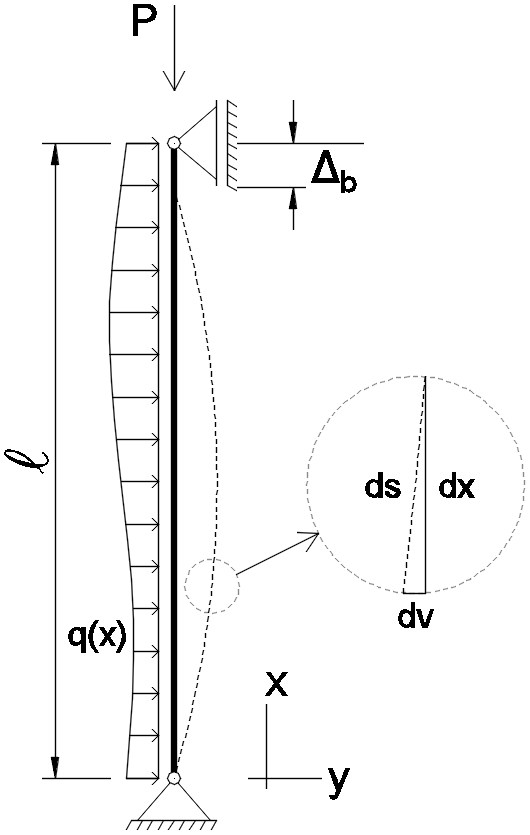
\includegraphics[width=0.3\textwidth]{confdef}
	\caption{Esquema de columna en configuraciones de referencia y deformada.}
	\label{fig:confdef}
\end{figure}

La energía potencial de deformación de la columna (o viga) está dada por:
%
\begin{equation}
\Pi_{int} = \frac{1}{2} \int_\Omega \bfsig : \bfvarep  \dif V  = \frac{1}{2} \int_\Omega \sigma_x \varepsilon_x  \dif V,
\end{equation}
%
donde sustituyendo las Ecuaciones \eqref{eqn:eccons} y \eqref{eqn:expdef} y usando que se desprecia energía de deformación axial $\varep_G$, se tiene:
%
\begin{equation}
\boxed{
\Pi_{int} = \frac{1}{2} \int_0^\ell \int_{A(x)} E(x) y^2 \left( \frac{\partial^2 v}{\partial x^2}\right)^2  \dif A \dif x 
=   \frac{1}{2} \int_0^\ell EI(x)  \left( \frac{\partial^2 v}{\partial x^2}\right)^2 \dif x.
}
\end{equation}

Se debe ahora obtener una expresión de la energía potencial de las fuerzas externas, como:
\begin{equation}
\Pi_{ext} = -P \Delta_b  - \int_0^\ell q(x) v(x) \dif x.
\end{equation}
%
donde $v(x)$ representa el desplazamiento según $y$ de la sección que en la configuración de referencia está ubicada en la posición $x$, y por lo tanto $x\in[0,\ell]$.



\subsubsection{Término de mayor orden}

Tal como se mencionó, el mayor orden y la capacidad de modelar con grandes desplazamientos es introducido en el término de energía potencial de las fuerzas externas, en particular, a través de la consideración de grandes desplazamientos en el descenso $\Delta_b$. %
%
A partir de asumir que $v$ no es pequeño, se observa que efectivamente se produce un descenso por la deformación de la columna (incluso sin considerar deformación axial). Integrando la deformada de la curva se tiene:
%
\begin{equation}
\Delta_b = \ell - \int_{\mathscr{C}_d} dx = \ell - \int_{\mathscr{C}_d} \sqrt{ds^2-dv^2} = \ell - 
\int_{\mathscr{C}_d} \sqrt{1-\left(\frac{\partial v}{\partial s}\right)^2} \dif s.
\end{equation}

El descenso $\Delta_b$ puede ser visto como una función no lineal de la función de flecha $v$:
%
$$
\Delta_b(v) = \ell - 
\int_{\mathscr{C}_d} \sqrt{1-\left(\frac{\partial v}{\partial s}\right)^2} \dif s.
$$

Es posible por lo tanto, establecer y aplicar un orden de aproximación para esta función, en el caso de aplicar primer orden se puede mostrar que $\Delta_b=0$, lo que sería coherente con la teoría lineal. %
%

En el caso de establecer una \textbf{aproximación de segundo orden} se puede aplicar un desarrollo de Taylor respecto al origen, obteniendo:
%
\begin{equation}\label{eqn:deltab}
\Delta_b \approx \ell - \int_{\mathscr{C}_d} \left[1 - \frac{1}{2}\left(\frac{\partial v}{\partial s}\right)^2\right] \dif s = \frac{1}{2} \int_0^\ell \left(\frac{\partial v}{\partial x}\right)^2 \dif x.
\end{equation}

Se tiene entonces que la energía potencial de las fuerzas $\Pi_{ext}$ puede ser aproximada por la siguiente expresión cuadrática en $v$:
%
\begin{equation}
\boxed{
\Pi_{ext} = -\frac{1}{2} P \int_0^\ell  \left(\frac{\partial v}{\partial x}\right)^2 \dif x - \int_0^\ell q(x) v(x) \dif x
}
\end{equation}

Obteniendo que la expresión de la energía potencial total es,
%
\begin{equation}\label{eqn:energiatotal}
\boxed{
\Pi(v) =  \frac{1}{2} \int_0^\ell EI(x) \left( \frac{\partial^2 v}{\partial x^2}\right)^2 \dif x -\frac{1}{2} P \int_0^\ell  \left(\frac{\partial v}{\partial x}\right)^2 \dif x - \int_0^\ell q(x) v(x) \dif x,
}
\end{equation}
donde se puede observar que esta función (u operador) es cuadrático en $v$ con un nuevo término respecto al desarrollo de la teórica lineal.

\subsubsection{Variación y condición de punto crítico}

Se deben encontrar las condiciones que debe cumplir la función $v(x)$ para minimizar la energía potencial total mostrada en la Ecuación~\ref{eqn:energiatotal}. %
%
Para esto se aplican de forma selectiva herramientas de \textit{calculo variacional}. El lector interesado puede consultar textos como \citep{Reddy2002b} o \citep{Taroco2019}.

La condición de que $v$ cumpla con la Ecuación~\ref{eqn:minPi} implica que ante variaciones pequeñas en $v$ la energía potencial total no varía, es decir que se tiene un punto crítico. %
%
Para obtener estas condiciones se considera una función arbitraria $\eta(x)$ diferenciable con derivada segunda continua, tal que al ser sumada a $v$ se obtiene una nueva función de flecha $\bar{v}$ que también cumple las condiciones de contorno
%
\begin{equation}\label{eqn:funcionv}
\bar{v}(x)=v(x)+\varepsilon\eta(x) \qquad \bar{v}\in \mcU,
\end{equation}
donde $\varepsilon$ es un real pequeño arbitrario. %
%
Se puede mostrar que $\eta$ debe cumplir condiciones de contorno homogéneas.

La expresión anterior representa una pequeña perturbación arbitraria de la deformación de la columna respecto de la configuración de equilibrio representada en la \autoref{fig:perturbacion}.
%
\begin{figure}[htb]
	\centering
	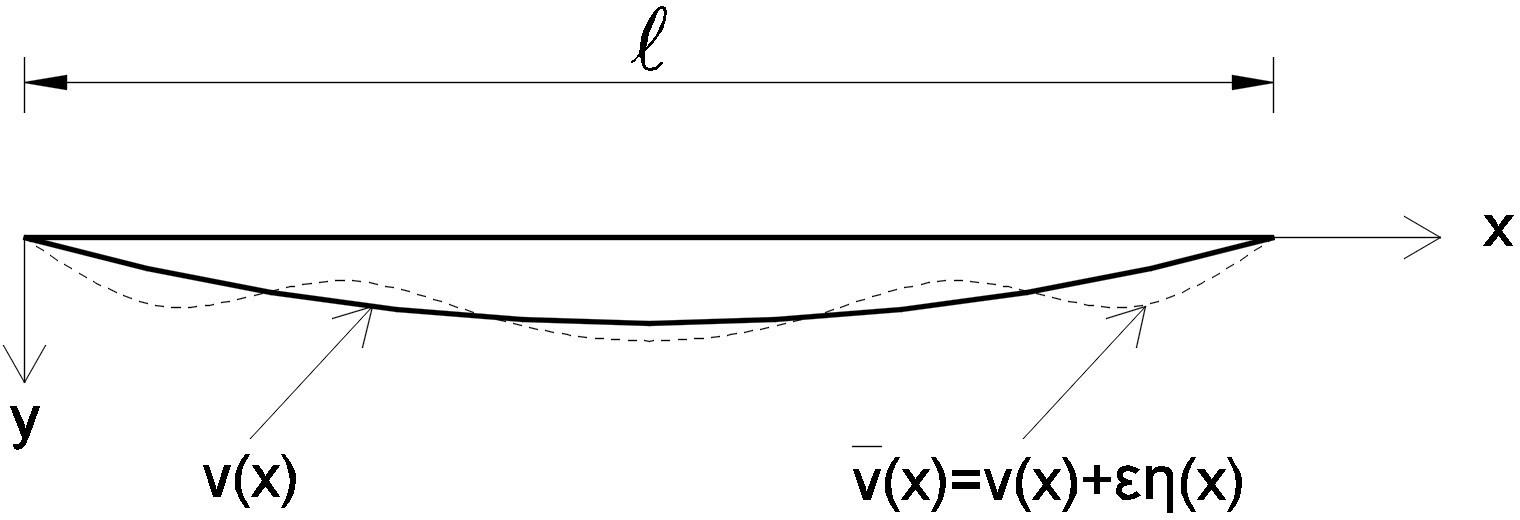
\includegraphics[width=0.55\textwidth]{perturbacion}
	\caption{Perturbación arbitraria de la deformación.}
	\label{fig:perturbacion}
\end{figure}

Si se sustituye la expresión \eqref{eqn:funcionv} en la Ecuación \eqref{eqn:energiatotal} se obtiene que la energía potencial para un desplazamiento arbitrario $\bar{v}(x)$ es

\begin{equation}\label{eqn:energiatotal2}
\Pi = \int_0^\ell \left[ \frac{EI}{2} \left( \frac{\partial^2 v}{\partial x^2} + \varepsilon\frac{\partial^2 \eta}{\partial x^2} \right)^2 - \frac{P}{2} \left(\frac{\partial v}{\partial x} + \varepsilon\frac{\partial \eta}{\partial x}\right)^2- q(x) \left( v(x)+\varepsilon\eta(x)\right) \right] \dif x
\end{equation}

La condición de Energía Potencial Interna estacionaria en $v(x)$ es equivalente a imponer que para toda perturbación $\eta(x)$ admisible no se debe tener variación en la energía. Esto es expresado como:
%
\begin{equation}
\frac{d\Pi}{d\varepsilon} \Bigg|_{\varepsilon=0} = 0 \quad \forall \eta .
\end{equation}

A partir de la Ecuación \eqref{eqn:energiatotal2} se obtiene,
\begin{equation}
\frac{d\Pi}{d\varepsilon} = \int_0^\ell \left[ EI \left( \frac{\partial^2 v}{\partial x^2} + \varepsilon\frac{\partial^2 \eta}{\partial x^2} \right) \frac{\partial^2 \eta}{\partial x^2} - P \left(\frac{\partial v}{\partial x} + \varepsilon\frac{\partial \eta}{\partial x}\right)\frac{\partial \eta}{\partial x}- q(x) \eta(x) \right] \dif x
\end{equation}

Sustituyendo $\varepsilon=0$ e imponiendo la condición de punto crítico se obtiene,
%
\begin{equation}\label{eqn:difenergia}
\frac{d\Pi}{d\varepsilon} \Bigg|_{\varepsilon=0} = \int_0^\ell \left[ EI \frac{\partial^2 v}{\partial x^2} \frac{\partial^2 \eta}{\partial x^2} - P \frac{\partial v}{\partial x}\frac{\partial \eta}{\partial x}- q(x) \eta(x) \right] \dif x = 0 \qquad \forall \eta
\end{equation}

Para simplificar la Ecuación \eqref{eqn:difenergia} se aplica integración por partes y las condiciones de contorno homogéneas de $\eta$ $\eta(0)=\eta(\ell)=0$. %
%
Se tiene entonces que para el segundo término de la Ecuación \eqref{eqn:difenergia},
%
\begin{equation}\label{eqn:partes1}
\int_0^\ell \frac{\partial v}{\partial x} \frac{\partial \eta}{\partial x}\dif x = \frac{\partial v}{\partial x}\eta\Bigg|_0^\ell - \int_0^\ell \frac{\partial^2 v}{\partial x^2} \eta\dif x 
= -\int_0^\ell \frac{\partial^2 v}{\partial x^2} \eta\dif x
\end{equation}

Por otra parte para el primer término de la Ecuación \eqref{eqn:difenergia} integrando por parte una vez se tiene,
%
$$
\int_0^\ell EI\frac{\partial^2 v}{\partial x^2} \frac{\partial^2 \eta}{\partial x^2}\dif x %
%
= EI\frac{\partial^2 v}{\partial x^2} \frac{\partial \eta}{\partial x}\Bigg|_0^\ell - \int_0^\ell \frac{\partial}{\partial x} \left( EI\frac{\partial^2 v}{\partial x^2} \right) \frac{\partial \eta}{\partial x}\dif x %
$$
e integrando nuevamente y usando la condición de contorno homogénea de $\eta$ se tiene
%
\begin{equation}\label{eqn:partes2}
\int_0^\ell EI\frac{\partial^2 v}{\partial x^2} \frac{\partial^2 \eta}{\partial x^2}\dif x %
%
= EI\frac{\partial^2 v}{\partial x^2} \frac{\partial \eta}{\partial x}\Bigg|_0^\ell %
%
+ \int_0^\ell \frac{\partial^2}{\partial x^2} \left( EI \frac{\partial^2 v}{\partial x^2} \right) \eta\dif x
\end{equation}

Sustituyendo las Ecuaciones \eqref{eqn:partes1} y \eqref{eqn:partes1} en la Ecuación \eqref{eqn:difenergia} se obtiene,

\begin{equation}\label{eqn:difenergia2}
\int_0^\ell \left[ \frac{\partial^2}{\partial x^2} \left(  EI \frac{\partial^2 v}{\partial x^2} \right) + P \frac{\partial^2 v}{\partial^2 x} - q(x)  \right] \eta(x) \dif x + EI\frac{\partial^2 v}{\partial x^2} \frac{\partial \eta}{\partial x}\Bigg|_0^\ell = 0
\end{equation}

%Recordar que esta condición debe cumplirse para todo $\eta(x)$ admisible, por lo tanto
%%
%$$
%\eta(x)\neq0 
%\qquad
%\frac{\partial \eta(0)}{\partial x} \neq 0
%\qquad
%\frac{\partial \eta(\ell)}{\partial x} \neq 0
%\qquad 
%\frac{\partial \eta(0)}{\partial x} \neq \frac{\partial \eta(\ell)}{\partial x}
%$$

La condición anterior debe cumplirse para cualquier función $\eta$ arbitraria, por lo que necesariamente deben cumplirse las siguientes condiciones:
%
\begin{eqnarray}
\frac{\partial^2}{\partial x^2} \left( EI \frac{\partial^2 v}{\partial x^2}(x) \right) + P \frac{\partial^2 v}{\partial^2 x}(x) - q(x) = 0 \qquad \text{Ecuación Euler-Lagrange} \label{eqn:euler} \\
EI\frac{\partial^2 v}{\partial x^2}\Bigg|_{x=0}=0 \qquad \text{Condición de contorno} \label{eqn:contorno1} \\
EI\frac{\partial^2 v}{\partial x^2}\Bigg|_{x=\ell}=0 \qquad \text{Condición de contorno} \label{eqn:contorno2}
\end{eqnarray}

Si bien las condiciones de contorno se impusieron al principio, se puede mostrar que estas condiciones no son estrictamente necesarias y que se puede obtener la misma ecuación diferencial que gobierna el problema \eqref{eqn:euler} para otras condiciones de contorno.

Por otra parte resulta de interés mostrar que la aplicación de la relación de la Ecuación~\eqref{eqn:eqcortante} en la Ecuación \eqref{eqn:euler} permite obtener una expresión para el cortante:
%
\begin{equation}\label{eqn:condcortante}
V(x) =
\frac{\partial}{\partial x} \left( EI \frac{\partial^2 v}{\partial x^2}(x) \right) + P \frac{\partial v}{\partial x}(x)
\end{equation}

También se recuerda la Ecuación \eqref{eqn:momen},  
\begin{equation}\label{eqn:condmomento}
M_z (x) = E I \frac{\partial^2 v}{\partial x^2}(x)
\end{equation}

\subsection{Solución Ecuación Homogénea}

La Ecuación \eqref{eqn:euler} es una ecuación de cuarto orden, lineal con un término independiente $q(x)$. Su solución estará compuesta por dos términos,
\begin{equation}
v(x)= v_p(x) + v_h(x)
\end{equation}

Donde $v_p(x)$ será una solución particular que dependerá de la carga distribuida $q(x)$ y $v_h(x)$ será la solución de la ecuación homogénea, esto es la solución de la ecuación diferencial cuando $q(x)=0$.

En este paso se establece una hipótesis frecuente en análisis de pórticos $EI$ uniforme en todo el elemento de viga. %
%
Además se define un parámetro $k$ como:
%
\begin{equation}\label{eqn:defk}
k = \sqrt{\frac{P}{EI}}
\end{equation}

De esta manera la Ecuación \eqref{eqn:euler} se puede reescribir como,
\begin{equation}\label{eqn:ecuahom}
\boxed{
\frac{\partial^4 v}{\partial x^4}(x) + k^2 \frac{\partial^2 v}{\partial^2 x}(x) = 0
}
\end{equation}

Utilizando un cambio de variable $\hat{v}=\frac{\partial^2 v}{\partial x^2}$ y sustityendo en la Ecuación~\eqref{eqn:ecuahom} se tiene
$$
\frac{\partial^2 \hat{v}}{\partial x^2}(x) + k^2 \hat{v}(x) = 0
$$
por lo que la solución homogénea sería
$$
\hat{v}(x) = \hat{A} \cos (kx) + \hat{B} \sin (kx).
$$

Deshaciendo el cambio de variable, es decir, integrando esta solución se tiene la expresión de la solución de la ecuación homogénea $v$:
%
\begin{equation}
v_h(x) = A \cos (kx) + B \sin (kx) + Cx + D
\end{equation}
%
donde las constantes multiplicando $\cos$ y $\sin$ fueron renombradas y las constantes $A$, $B$, $C$ y $D$ deben determinarse empleando las condiciones de contorno sobre la solución particular en cada problema como se verá en la Sección~\ref{sec:componentes}.


\subsection{Límites de la teoría}

Es importante destacar que esta teoría tiene un límite de aplicación acotado. La teoría es aplicable mientras que la aproximación realizada en la Ecuación~\ref{eqn:deltab} mantenga validez. %
%
Esta teoría puede ser mejorada considerando modelos estructurales que permitan evaluar grandes rotaciones de elementos y grandes desplazamientos. En dicho caso se podrían incorporar expresiones exactas de la cinemática de la estructura. %
%
Un ejemplo típico de esto es la curvatura exacta de una viga, la cual en la hipótesis de pequeños giros fue simplifica por una derivada segunda de la deformación lateral de la viga.


\section{Estabilidad Elástica de Componentes} \label{sec:componentes}

En esta sección se obtienen las soluciones de la ecuación de pandeo para algunos casos de interés práctico.

\subsection{Columna de Euler}

La columna de Euler es un caso de gran relevancia tanto en el diseño de pilares así como también por su importancia en el desarrollo histórico de la temática.
%
La columna de Euler consiste en una columna de rigidez flexional uniforma $EI$ sometida a una carga de compresión según su eje, sin cargas transversales aplicadas, tal como se muestra en la Figura~\ref{fig:euler}.

\begin{figure}[htb]
	\centering
	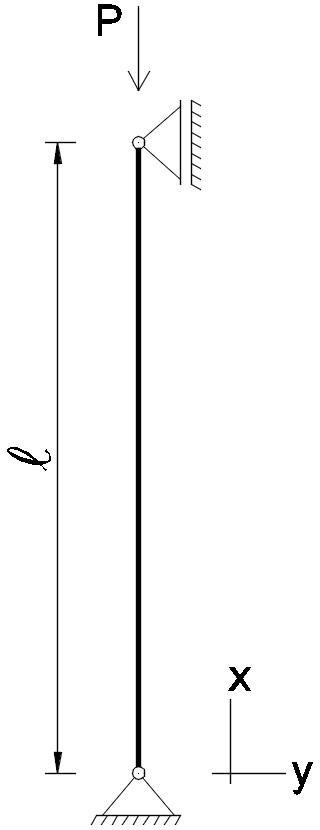
\includegraphics[width=0.15\textwidth]{euler}
	\caption{Esquema de columna de Euler.}
	\label{fig:euler}
\end{figure}

La ecuación diferencial de la deflexión $v$ está dada por la Ecuación~\eqref{eqn:ecuahom} y la solución y sus derivadas están dadas por:
%
\begin{eqnarray}
v(x) &=& A \cos(k x ) + B \sin(kx) + C x + D, \\
\frac{\partial   v}{\partial x  } (x) &=& -A k \sin(k x ) + B k \cos(kx) + C , \\
\frac{\partial^2 v}{\partial x^2} (x) &=& - A k^2 \cos(k x ) - B k^2 \sin(kx)
\end{eqnarray}
con $k$ dado por la Ecuación~\eqref{eqn:defk}.

Las condiciones de contorno en función de las flechas o solicitaciones son,
%
\begin{equation}
\left\{
\begin{array}{l}
v(0)=0 \\[.5em]
\displaystyle v(\ell)=0\\[.5em]
M(0)=0\\[.5em]
M(\ell)=0
\end{array}
\right.
\end{equation}

Aplicando las condiciones anteriores se tiene:
%
\begin{eqnarray}
v(0) &=& 0 \Rightarrow A + D = 0, \\
v(\ell) &=& 0 \Rightarrow A \cos(k \ell) + B \sin(k \ell) + C \ell + D = 0, \\
M(0) &=& EI \frac {\partial^2 v}{\partial x^2} (0) = 0 \Rightarrow -Ak^2 = 0,  \\
M(\ell) &=& EI \frac{\partial^2 v}{\partial x^2} (\ell) = 0  \Rightarrow -Ak^2\cos(k \ell) -  B k^2 \sin(k\ell) = 0,
\end{eqnarray}

De las ecuaciones anteriores y teniendo en cuenta que $k>0$ se obtiene que se deben cumplir las siguientes condiciones
\begin{equation}
A = B\sin(k\ell) = C = D = 0
\end{equation}

Por lo tanto existen dos alternativas, $A = B = C = D = 0$, que es la solución trivial ya conocida o que $\sin(k\ell) = 0$.
Para que esto último se cumpla se tiene que,
\begin{equation}
k \ell = n \pi  \quad \text{con} \,\, n\in \bbN
\end{equation}

En ese caso cualquier valor de $B$ cumple la condición por lo que existen infinitas soluciones. En particular la menor directa asociada a estos valores de $k$ es con $n=1$,
\begin{equation}\label{eqn:criticaeuler}
\boxed{P_{cr} = \frac{\pi^2 E I}{\ell^2}}
\end{equation}
Siendo esta la expresión de la Carga Crítica que produce la inestabilidad en la Columna de Euler.

\subsection{Luz de Pandeo}

Se considera $\ell$ como la luz libre del elemento en estudio, se define entonces $L_P$ como la luz de pandeo de dicho elemento, como
\begin{equation}
L_P=\beta\ell
\end{equation}
Donde $\beta$ depende de los vínculos que tenga el elemento. De esta manera la expresión de Carga Crítica \eqref{eqn:criticaeuler} se puede generalizar como,
\begin{equation}\label{eqn:criticageneral}
\boxed{P_{cr} = \frac{\pi^2 E I}{L_P^2}}
\end{equation}

Para un elemento simplemente apoyado se determinó que la Carga Crítica es,
$$P_{cr} = \frac{\pi^2 E I}{\ell^2}$$
mientras que para un elemento en ménsula, con un extremo empotrado y otro libre, se verá mas adelante que la Carga Crítica es,
$$P_{cr} = \frac{\pi^2 E I}{4\ell^2}$$
Se observa que para el caso del elemento simplemente apoyado la luz de pandeo es $L_P=\ell$ y por lo tanto $\beta=1$, mientras que para el caso del elemento en ménsula la luz de pandeo es $L_P=2\ell$ y por lo tanto $\beta=2$. 

Se puede observar en la Figura~\ref{fig:luzpandeo} que el caso del elemento en ménsula puede ser asimilado al caso de un elemento simplemente apoyado de longitud $2\ell$. Resolviendo analíticamente otros casos y realizando un razonamiento similar se puede ver que la luz de pandeo es también la distancia entre dos puntos de momento nulo. Esto último implica que la longitud de pandeo también se puede interpretar como aquella que separa puntos con curvatura acotada, debido a que los puntos de momento nulo coinciden con los puntos de inflexión de la elástica.

\begin{figure}[htb]
	\centering
	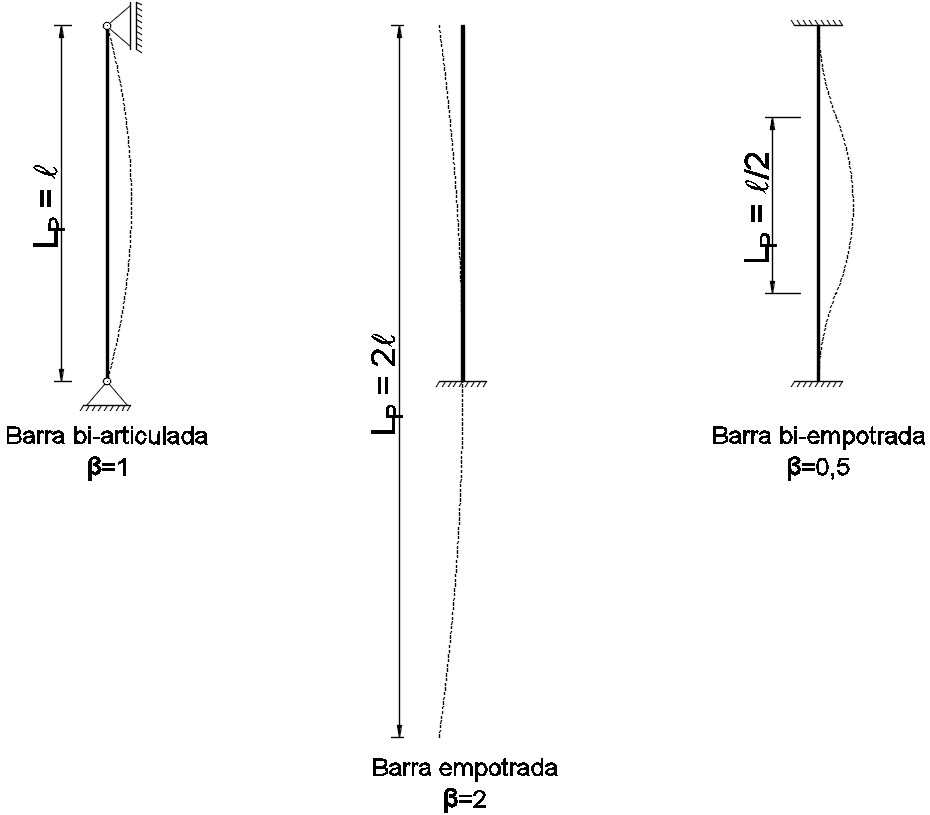
\includegraphics[width=0.6\textwidth]{LuzPandeo}
	\caption{Luz de Pandeo según condiciones de apoyo.}
	\label{fig:luzpandeo}
\end{figure}

\subsection{Esbeltez}

Se define la esbeltez $\lambda$ de un elemento comprimido de la siguiente manera,
\begin{equation}
\lambda = \frac{L_P}{\rho}
\end{equation}

Donde el radio de giro $\rho$ de la sección respecto de un eje principal cumple que
\begin{equation}
\rho^2 = \frac{I}{A},
\end{equation}
tal como se vió en la Sección~\ref{sec:lnnc}.

Si se sustituye en la Ecuación \eqref{eqn:criticageneral} se tiene
$$
P_{cr} = \frac{\pi^2 E A \rho^2}{L_P^2} = \frac{\pi^2 E A}{\left(\frac{L_P}{\rho}\right)^2}
$$

Obteniendo que,
\begin{equation}
\boxed{P_{cr} = \frac{\pi^2 E A}{\lambda^2}}
\end{equation}

De igual manera y usando que $\sigma=P/A$ se puede definir una tensión de compresión crítica como  
\begin{equation}
\boxed{\sigma_{cr} = \frac{\pi^2 E}{\lambda^2}}
\end{equation}
Cuyo valor tiene como cota superior la tensión admisible $\sigma_{adm}$ del material.

Hasta ahora se ha estudiado el fenómeno de pandeo con propiedades geométricas $I$ y $\rho$ genéricas. Sin embargo, si los vínculos del elemento son iguales en ambas direcciones la carga crítica quedará determinada por el menor momento de inercia. Por otra parte, para analizar el fenómeno de pandeo en elementos con vínculos distintos en cada dirección, será necesario estudiar ambas direcciones por separado con el momento de inercia que corresponda, quedando en general determinado por la dirección de mayor esbeltez.

\subsection{Ejemplo: ménsula con carga axial}

Se considera una ménsula formada por un material de módulo de Young $E$, de largo $\ell$ con sección transversal de inercia $I$ sometida a una carga axial de compresión $N=P$ aplicada en su extremo libre con una excentricidad $e$, como se muestra en la Figura~\ref{fig:esqpand}. %
%
No hay carga transversal aplicada, por lo tanto $q=0$. %

\begin{figure}[htb]
\centering
\def\svgwidth{0.7\textwidth}
\input{figs/UT7/ejemplo_pandeo.pdf_tex}
\caption{Esquema de ménsula con carga axial con excentricidad.}
\label{fig:esqpand}
\end{figure}

En estructuras reales, excentricidades como la considerada $e$ pueden estar asociadas o ser causadas por errores en la ejecución de elementos estructurales conectados a la ménsula (por ejemplo vigas descargando sobre columnas). %
%
Esto permite considerar la excentricidad como una \textit{imperfección}, la cual usualmente tiene magnitud considerablemente menor a las dimensiones de la sección transversal. %
% ------------------------------------------

Como ya se vió, la ecuación diferencial de la deflexión $v$ en este caso está dada por
%
$$
  E I \frac{\partial^4 v}{\partial x^4}(x)
+   P \frac{\partial^2 v}{\partial x^2}(x)
=   0
$$

La solución y sus derivadas están dadas por:
\begin{eqnarray}
v(x) &=& A \cos(k x ) + B \sin(kx) + C x + D, \\
\frac{\partial   v}{\partial x  } (x) &=& -A k \sin(k x ) + B k \cos(kx) + C , \\
\frac{\partial^2 v}{\partial x^2} (x) &=& - A k^2 \cos(k x ) - B k^2 \sin(kx),  \\
\frac{\partial^3 v}{\partial x^3} (x) &=& A k^3 \sin(k x ) - B k^3 \cos(kx), 
\end{eqnarray}
con k según la Ecuación \eqref{eqn:defk}

Las condiciones de contorno en función de las flechas o solicitaciones son,
\begin{equation}
\left\{
\begin{array}{l}
v(0)=0 \\[.5em]
\displaystyle \frac{\partial v}{\partial x}(0)=0\\[1em]
V(\ell)=0\\[.5em]
M(\ell)=-P e
\end{array}
\right.
\end{equation}

Es necesario obtener las condiciones de contorno en función de la flecha. %
Se comienza desarrollando la condición del cortante, es decir,
%
\begin{equation}
	V(\ell) = 0,
\end{equation}
Utilizando la Ecuación \eqref{eqn:condcortante} y operando se obtiene la relación equivalente, en función de la flecha:
%
\begin{equation}
  \frac{\partial^3 v}{\partial x^3} (\ell) = - k^2 \frac{\partial v}{\partial x}(\ell).
\end{equation}
%
Sustituyendo la expresión de la solución se tiene:
%	
\begin{equation}
	Ak^3 \sin(k\ell) - Bk^3 \cos(k\ell) = Ak^3 \sin(k\ell) - Bk^3 \cos(k\ell) - C k^2,
\end{equation}
por lo tanto se cumple:
\begin{equation}\label{eqn:ejemplopand}
\boxed{
  C=0
}
\end{equation}

Usando la condición de giro nulo en el empotramiento se tiene
\begin{equation}
v'(0)=0 \Leftrightarrow  Bk + C = 0,
\end{equation}
%
por lo tanto usando la Ecuación~\eqref{eqn:ejemplopand} se tiene
\begin{equation}
\boxed{
B=0
}
\end{equation}

Usando la Ecuación \eqref{eqn:condmomento} y la condición de momento en $\ell$ se tiene
%
\begin{equation}
M(\ell) = -P e \Leftrightarrow \frac{\partial v^2}{\partial x^2} (\ell)  = - k^2 e
\end{equation}
%
por lo tanto
%
\begin{equation}
-k^2 A \cos(k\ell) - k^2 B \cos(k\ell) = -k^2 e
\end{equation}

Esto es equivalente a 
\begin{equation}\label{eqn:acos}
\boxed{
A \cos(k\ell)  = e
}
\end{equation}

Finalmente usando la condición de desplazamiento nulo en el empotramiento se tiene
%
\begin{equation}
v(0)=0  \Leftrightarrow \boxed{ A + D = 0}
\end{equation}

Es necesario estudiar de forma independiente las soluciones obtenidas para los casos con y sin imperfecciones.

\subsubsection{Solución sin imperfección}

El caso sin imperfección corresponde a $e=0$ y la expresión solución está dada por:
%
\begin{equation}
v(x) = A (\cos(k x) -1), \quad \text{con} \quad A\cos(k\ell) = 0.
\end{equation}

Si se verifica
%
\begin{equation}
k \ell = \frac{\pi}{2} + n\pi  \quad \text{con} \,\, n\in \bbN,
\end{equation}
%
entonces cualquier valor de $A$ cumple la condición por lo que existen infinitas soluciones. %
%
En particular la menor directa asociada a estos valores de $k$ es
\begin{equation}
\boxed{
P_{cr} = \frac{\pi^2 E I}{4 \ell^2}}
\end{equation}
%
Esta carga crítica corresponde a una luz de pandeo $L_p = 2\ell$.

\subsubsection{Solución con imperfección}

En este caso se considera una excentricidad $e \neq 0$, por lo que se obtiene una única solución dada por:
%
\begin{equation}
v(x) = \frac{e}{\cos(k\ell)} (\cos(k x) -1).
\end{equation}
%
Se destaca que se asumió que $\cos(k \ell) \neq 0$, en caso contrario se tendría una incompatibilidad en la Ecuación~\eqref{eqn:acos}. %

Se mostrará que, de acuerdo con el modelo considerado, existe un nivel de carga para el cual la estructura pierde capacidad de soportar cargas superiores (rigidez) y la flecha adquiere valores elevados. %
%

Como referencia se considera la flecha en el extremo libre, es decir:
%
\begin{equation}
v(\ell) = e \left( 1- \frac{1}{\cos(k\ell) }  \right)
\end{equation}
%
si $k=0$ se tiene un valor nulo de flecha, mientras que al aumentar el valor de $P$ se tiene un crecimiento que lleva a que cuando se alcanza el valor 
%
\begin{equation}
k = \frac{\pi}{2 \ell }
\end{equation}
%
la flecha tiende a infinito. %
%
Esto establece por lo tanto que la carga crítica de la estructura es la misma del caso anterior
%
\begin{equation}
\boxed{
	P_{cr} = \frac{\pi^2 E I}{4 \ell^2}.
}
\end{equation}


En la Figura~\ref{fig:ejpand} se presenta la curva de desplazamientos del extremo libre (abscisas) para diferentes valores de $k\ell$ (ordenadas). %
%
Para $k\ell$ se consideran 30 valores equiespaciados entre $0$ y $\frac{\pi}{2} 0.99$.

\begin{figure}[htb]
	\centering
		\resizebox{.7\textwidth}{!}{% Title: gl2ps_renderer figure
% Creator: GL2PS 1.3.9, (C) 1999-2015 C. Geuzaine
% For: Octave
% CreationDate: Mon Dec  4 08:08:25 2017
\setlength{\unitlength}{1pt}
\begin{picture}(0,0)
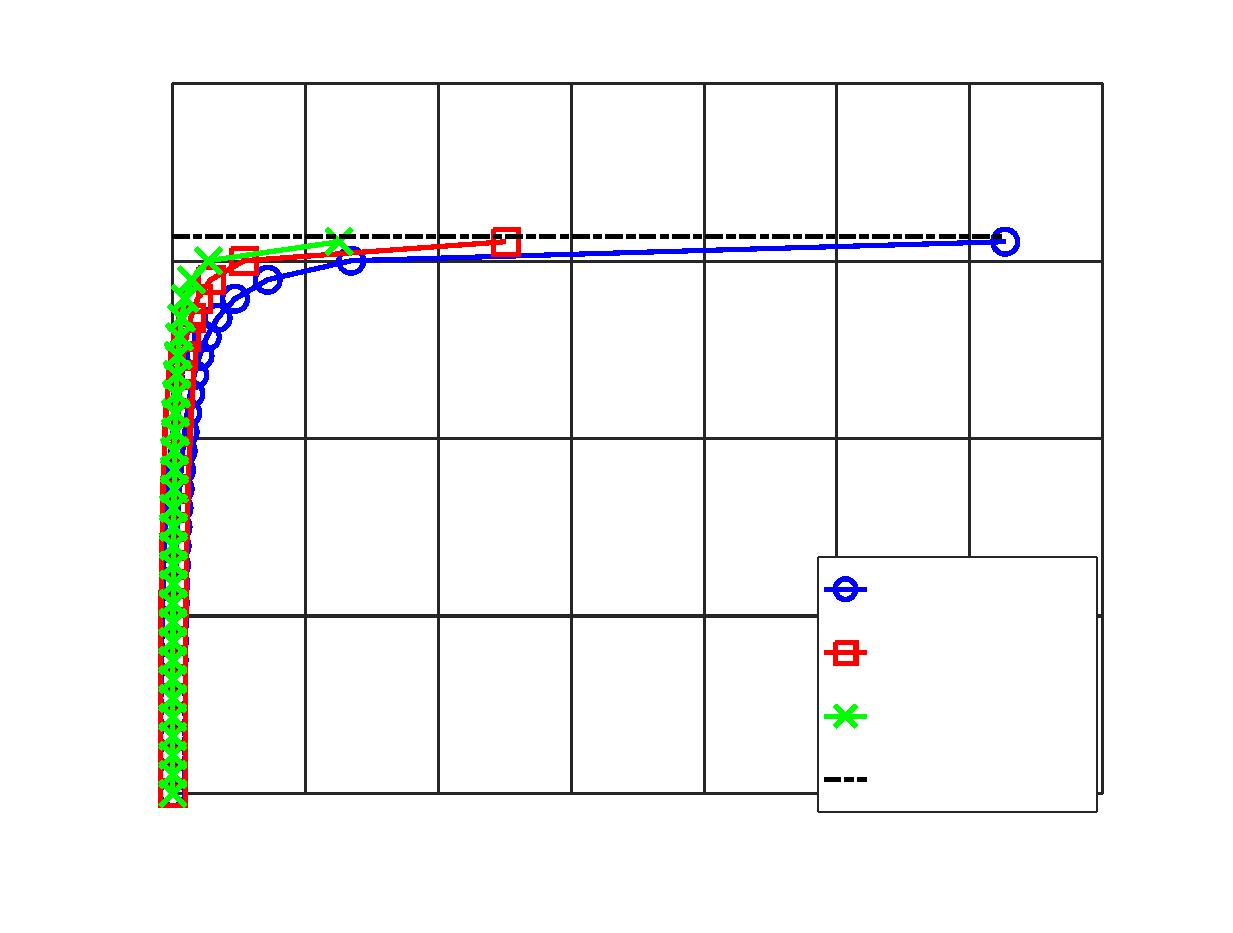
\includegraphics{plotejempand-inc}
\end{picture}%
\begin{picture}(576,432)(0,0)
\fontsize{22}{0}
\selectfont\put(74.88,54.0046){\makebox(0,0)[t]{\textcolor[rgb]{0.15,0.15,0.15}{{0}}}}
\fontsize{22}{0}
\selectfont\put(138.651,54.0046){\makebox(0,0)[t]{\textcolor[rgb]{0.15,0.15,0.15}{{5}}}}
\fontsize{22}{0}
\selectfont\put(202.423,54.0046){\makebox(0,0)[t]{\textcolor[rgb]{0.15,0.15,0.15}{{10}}}}
\fontsize{22}{0}
\selectfont\put(266.194,54.0046){\makebox(0,0)[t]{\textcolor[rgb]{0.15,0.15,0.15}{{15}}}}
\fontsize{22}{0}
\selectfont\put(329.966,54.0046){\makebox(0,0)[t]{\textcolor[rgb]{0.15,0.15,0.15}{{20}}}}
\fontsize{22}{0}
\selectfont\put(393.737,54.0046){\makebox(0,0)[t]{\textcolor[rgb]{0.15,0.15,0.15}{{25}}}}
\fontsize{22}{0}
\selectfont\put(457.509,54.0046){\makebox(0,0)[t]{\textcolor[rgb]{0.15,0.15,0.15}{{30}}}}
\fontsize{22}{0}
\selectfont\put(521.28,54.0046){\makebox(0,0)[t]{\textcolor[rgb]{0.15,0.15,0.15}{{35}}}}
\fontsize{22}{0}
\selectfont\put(69.8755,58.9987){\makebox(0,0)[r]{\textcolor[rgb]{0.15,0.15,0.15}{{0}}}}
\fontsize{22}{0}
\selectfont\put(69.8755,144.149){\makebox(0,0)[r]{\textcolor[rgb]{0.15,0.15,0.15}{{0.5}}}}
\fontsize{22}{0}
\selectfont\put(69.8755,229.299){\makebox(0,0)[r]{\textcolor[rgb]{0.15,0.15,0.15}{{1}}}}
\fontsize{22}{0}
\selectfont\put(69.8755,314.45){\makebox(0,0)[r]{\textcolor[rgb]{0.15,0.15,0.15}{{1.5}}}}
\fontsize{22}{0}
\selectfont\put(69.8755,399.6){\makebox(0,0)[r]{\textcolor[rgb]{0.15,0.15,0.15}{{2}}}}
\fontsize{22}{0}
\selectfont\put(298.08,27.0046){\makebox(0,0)[t]{\textcolor[rgb]{0.15,0.15,0.15}{{Desplazamiento $v(\ell)$}}}}
\fontsize{22}{0}
\selectfont\put(30.8755,229.299){\rotatebox{90}{\makebox(0,0)[b]{\textcolor[rgb]{0.15,0.15,0.15}{{$k \ell$}}}}}
\fontsize{22}{0}
\selectfont\put(410.88,157.064){\makebox(0,0)[l]{\textcolor[rgb]{0,0,0}{{$e=$ 0.5}}}}
\fontsize{22}{0}
\selectfont\put(410.88,126.549){\makebox(0,0)[l]{\textcolor[rgb]{0,0,0}{{$e=$ 0.2}}}}
\fontsize{22}{0}
\selectfont\put(410.88,96.0347){\makebox(0,0)[l]{\textcolor[rgb]{0,0,0}{{$e=$ 0.1}}}}
\fontsize{22}{0}
\selectfont\put(410.88,65.5203){\makebox(0,0)[l]{\textcolor[rgb]{0,0,0}{{$e=0$}}}}
\end{picture}
}
	\caption{Resultado analítico de inestabilidad con imperfección.}
	\label{fig:ejpand}
\end{figure}

Se puede observar cómo la presencia de imperfecciones de mayor magnitud provocan que la estructura tenga mayores desplazamientos para cada valor de carga dado. %
%
Para todas las excentricidades, la curva tiene una asíntota horizontal en $k\ell=\frac{\pi}{2}$, por lo que este modelo establece que la estructura no es capaz de soportar cargas superiores a la carga crítica.


La curvatura está dada por la función 
\begin{equation}
\frac{\partial^2 v}{\partial x^2}(x) = -k^2 e \frac{\cos(k x)}{\cos(k\ell)}.
\end{equation}


Se puede mostrar que
\begin{equation}
\lim\limits_{P\rightarrow P_{cr}}
\left| \frac{\partial^2 v}{\partial x^2}(x) \right|
 =
\left\{
\begin{array}{lr}
\infty & \text{si } x \in (-\ell,\ell)\\
\displaystyle \frac{\pi^2 e}{4 \ell^2} & \text{si } x \in \{-\ell,\ell\}
\end{array}
\right.
\end{equation}
%
por lo tanto, a partir de este resultado, se puede observar como la longitud de pandeo es aquella que separa puntos con curvatura acotada.


%\subsection{Otros Componentes}
% - (1c) Otros tipos de inestabilidad de componentes. Nombrar + Imagen (plot de Robot x ejemplo) y referir a Curso de Mecanica Estructural:
% * Inestabilidad torsional en columnas
% * Inestabilidad flexo-torsional en columnas
% * Inestabilidad lateral torsional en vigas

%\subsection{Inestabilidades Locales}
% - (1c) Inestabilidades en elementos de componentes referir a curso Estructuras de Acero:
% * Inestabilidad de alas y almas en compresión.
% * Inestabilidad de almas en corte.
% * Resistencia post-crítica de chapas planas permite tener capacidad más alla de carga crítica.



\newpage

\section{Ejercicios}
\setcounter{ejercicio}{0}

Nota: Salvo aclaración contraria, se considerará que las piezas pueden pandear en torno a cualquiera de sus direcciones principales.

\ejercicio 

Determinar los coeficientes $\beta$ tal que la luz de pandeo es $L_P=\beta\ell$ para las condiciones de borde mostradas en la Figura~\ref{fig:UT71}.

\begin{figure}[htb]
	\centering
	\subfloat[]{
		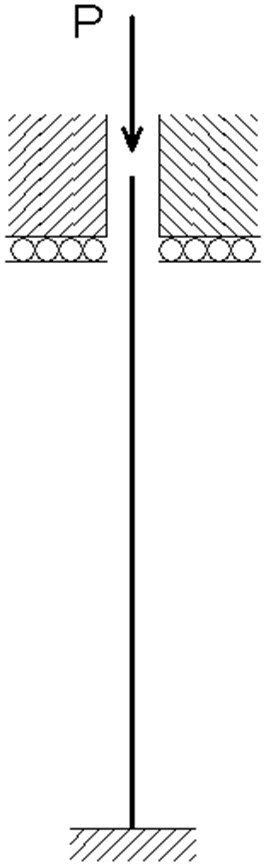
\includegraphics[width=0.1\textwidth]{UT7ej1-a}
		\label{fig:UT71.a}}
	\hspace{0.1\textwidth}
	\subfloat[]{
		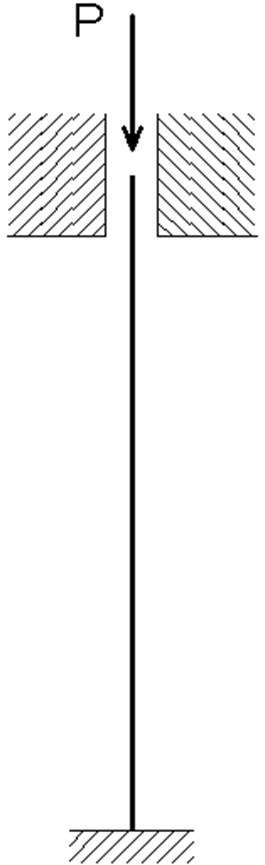
\includegraphics[width=0.1\textwidth]{UT7ej1-b}
		\label{fig:UT71.b}}
	\hspace{0.1\textwidth}
	\subfloat[]{
		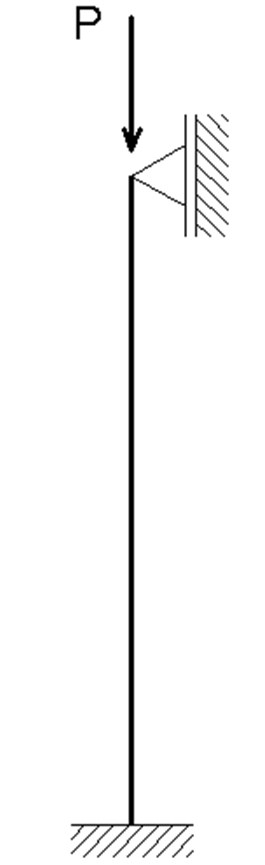
\includegraphics[width=0.1\textwidth]{UT7ej1-c}
		\label{fig:UT71.c}}
	\caption{Condiciones de borde a considerar en Ejercicio 7.1.}
	\label{fig:UT71}
\end{figure}

Sugerencia: para ~\ref{fig:UT71.a} y ~\ref{fig:UT71.c}, plantear el origen de coordenadas en el extremo superior del pilar.

%\ejercicio 
%
%Dada la barra de la Figura, construida con un $PNI30$, determinar $P_{cr}$ si $\sigma_{adm}=140MPa$, $E=200GPa$ y $L=2m$.
%
%\begin{center}
%	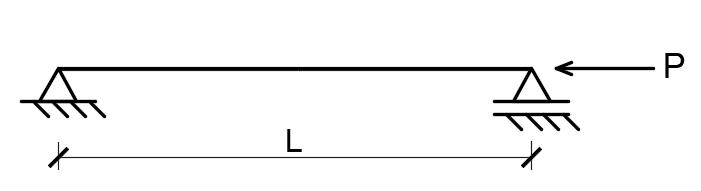
\includegraphics[width=0.5\linewidth]{UT7ej2}
%\end{center}

%\ejercicio 
%
%Dimensionar la barra de la Figura en sección cuadrada de madera, sabiendo que $\sigma_{adm}=10MPa$ y $E=10GPa$. Utilizar las tablas de escuadrías de madera.
%
%\begin{center}
%	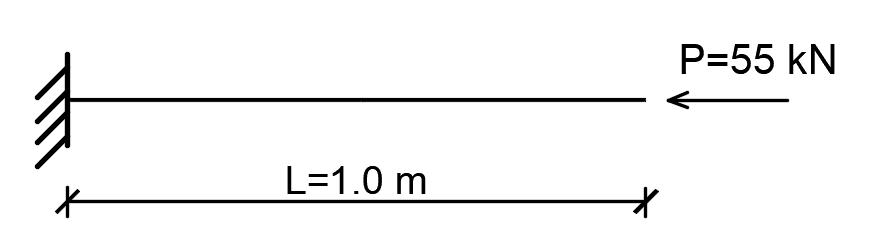
\includegraphics[width=0.5\linewidth]{UT7ej3}
%\end{center}

%\ejercicio 
%
%\begin{center}
%	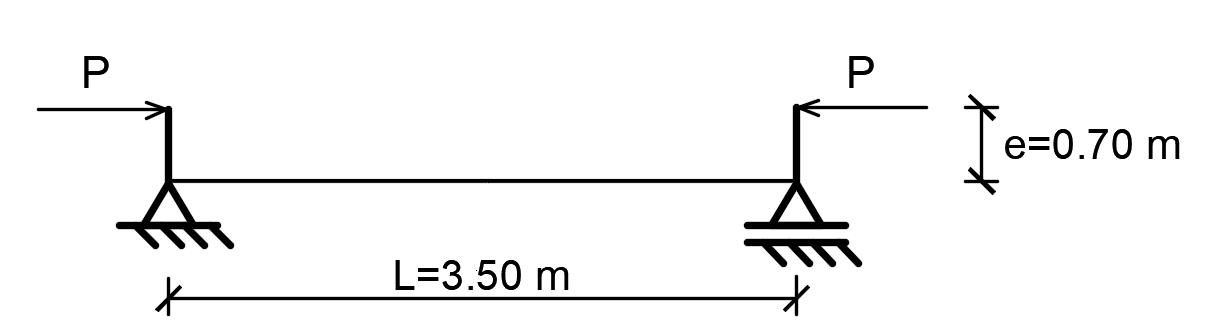
\includegraphics[width=0.6\linewidth]{UT7ej4-3}
%\end{center}
%
%Dada la barra de la estructura, construida con un $PNI14$ ($\sigma_{adm}=140MPa$ y $E=200GPa$), determinar $P_{cr}$ para los siguientes dos casos:
%
%\begin{figure}[htb]
%	\centering
%	\subfloat[Caso 1]{
%		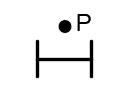
\includegraphics[width=0.2\textwidth]{UT7ej4-1}
%		\label{fig:UT74.1}}
%	~
%	\subfloat[Caso 2]{
%		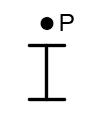
\includegraphics[width=0.15\textwidth]{UT7ej4-2}
%		\label{fig:UT74.2}}
%	\caption{}
%	\label{fig:UT74}
%\end{figure}

%\ejercicio
%
%\begin{minipage}[b]{0.7\textwidth}
%	
%	Una columna soldada de 8 m de luz tiene la sección de la figura conformada por acero ($\sigma_{adm}=140MPa$ y $E=200GPa$). 
%	\parte Hallar $x$ tal que el radio de giro de la sección según sus dos ejes sea el mismo, es decir que la sección trabaje de forma óptima.
%	\parte ¿Cuál es la carga de compresión crítica centrada si el esquema estructural de la columna es el de una ménsula?
%	
%\end{minipage}
%~
%\begin{minipage}[b]{0.3\textwidth}
%	\begin{center}
%		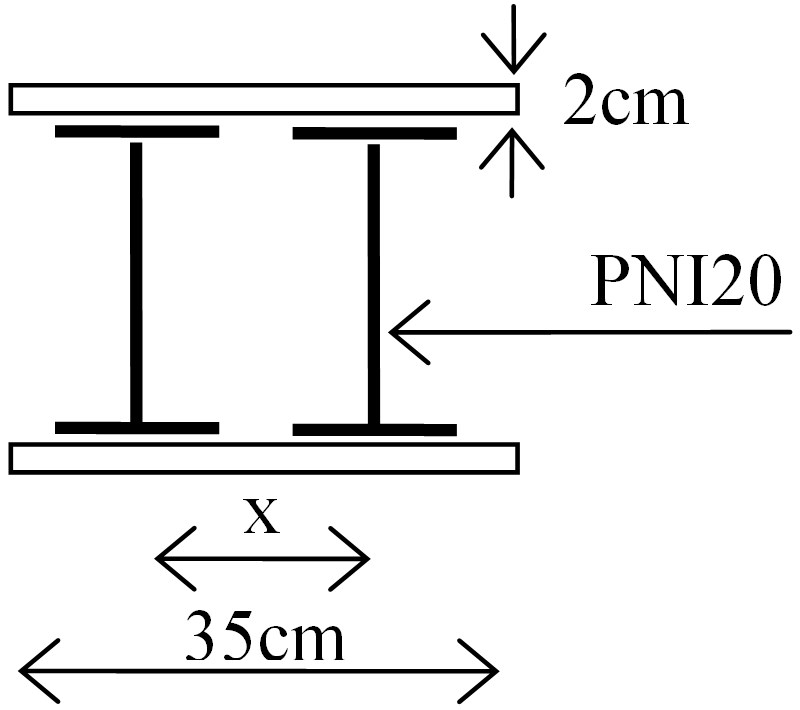
\includegraphics[width=0.85\linewidth]{UT7ej5}
%	\end{center}
%\end{minipage}





\ejercicio

La barra horizontal de la figura está soportada por dos columnas. Cada columna está articulada en su parte superior a la barra horizontal, mientras que el apoyo inferior de la columna izquierda es un empotramiento y el de la derecha es un apoyo fijo. Ambas columnas son barras de acero $E=200GPa$ de sección transversal cuadrada con un ancho de $15 mm$.
\parte Si $a=0.4m$, ¿Cuál es el valor crítico de la carga $Q$?
\parte Si $a$ varía entre 0 y 1 m. ¿Cuál es el valor máximo de $Q_{critico}$, y cuál es el valor correspondiente de $a$?

Nota: Estudiar la inestabilidad sólo en el plano de la figura.

\begin{center}
	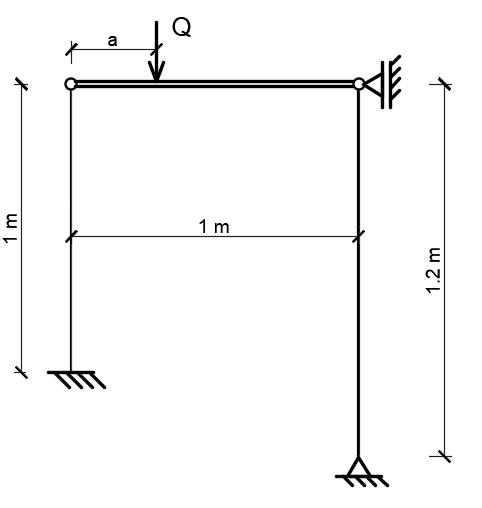
\includegraphics[width=0.4\linewidth]{UT7ej6}
\end{center}





\ejercicio

\begin{minipage}[b]{0.6\textwidth}
	
	Una columna rectangular, con dimensiones de sección transversal $b \times h$, está articulada en los extremos A y C, como se indica en la Figura.
	
	La columna está restringida en el plano de la figura en la mitad de su altura, pero puede deformarse libremente en el plano perpendicular al de la figura.
	
	Determinar la relación $h/b$ tal que la carga crítica sea la misma para el pandeo en los dos planos principales de la columna.
	
	Nota: Analizar el problema a partir de los posibles modos de pandeo obtenidos en un pilar biarticulado.
	
\end{minipage}
~
\begin{minipage}[b]{0.4\textwidth}
	\begin{center}
		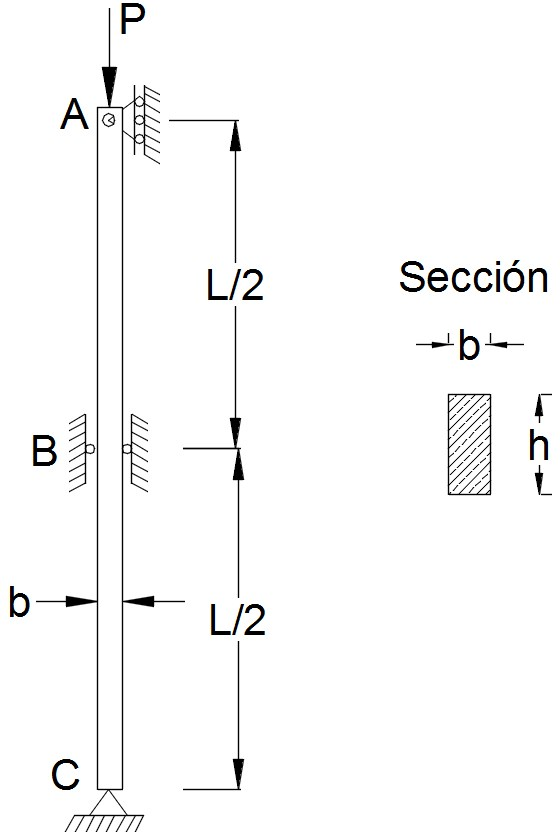
\includegraphics[width=0.65\linewidth]{UT7ej7}
	\end{center}
\end{minipage}





\ejercicio

Se tiene la columna de la Figura (con $EI$ uniforme) de largo $L$. La misma está soportada en su parte superior por un resorte elástico lineal de constante $r=2EI/L^3$ contenido en el $plano$ $xy$, mientras que en el plano perpendicular se encuentra en ménsula (libre en su extremo superior). Se pretende que la pieza sea capaz de soportar una carga $Q=200 kN$ con una altura $L=3m$.

Hallar la ecuación que permite determinar la luz de pandeo en el plano del resorte y demostrar que $L_p=1,56L$. Se sugiere plantear el origen de coordenadas en el extremo superior del pilar.

%\parte Dimensionar dicha pieza con un perfil laminado $PNI$ ($\sigma_{adm}=140MPa$ y $E=200GPa$).
%\parte Dimensionarla utilizando perfiles laminados $PNIP$ ($\sigma_{adm}=140MPa$ y $E=200GPa$). 
%\parte Dimensionarla utilizando una escuadría cuadrada de quebracho, el cual tiene una tensión admisible $\sigma_{adm,comp//}=12MPa$ (compresión paralela a las fibras) y $E=10GPa$.
%
%En b), c) y d) indicar como orientar el perfil o escuadría.

\begin{center}
	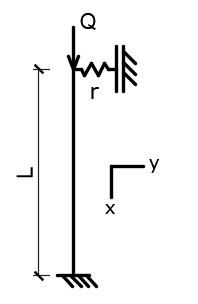
\includegraphics[width=0.22\linewidth]{UT7ej8}
\end{center}

%
%\ejercicio (Adicional)
%
%\begin{center}
%	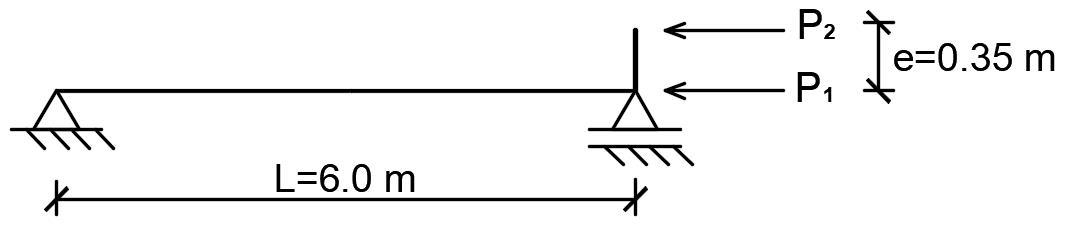
\includegraphics[width=0.6\linewidth]{UT7ej10-3}
%\end{center}
%
%Sean $P_1=500 kN$ y $P_2=120 kN$. Dimensionar en $PNIP$ (alas anchas) considerando $\sigma_{adm}=140MPa$ y $E=200GPa$. Analizar dos casos:
%
%\begin{figure}[htb]
%	\centering
%	\subfloat[Caso 1]{
%		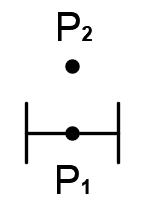
\includegraphics[width=0.15\textwidth]{UT7ej10-1}
%		\label{fig:UT710.1}}
%	~
%	\subfloat[Caso 2]{
%		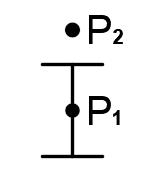
\includegraphics[width=0.15\textwidth]{UT7ej10-2}
%		\label{fig:UT710.2}}
%	\caption{}
%	\label{fig:UT710}
%\end{figure}
%


\ejercicio

Sea la siguiente estructura formada por barras de longitud $\ell$ y rigideces a flexión $EI_c$ y $EI_b$ sometida a una carga puntual $P$, como se muestra en la figura. Se asume que las barras tienen rigidez axial tal que no hay deformación axial (barras inextensibles).

\begin{center}
		\def\svgwidth{0.5\textwidth}
		\input{figs/UT7/ejPortL.pdf_tex}
\end{center} 

Se asume que al alcanzar la carga de pandeo, el cortante en la barra BC es despreciable con respecto a $P_{cr}$, es decir que es considerado $V_{BC} \approx 0$, por lo que se puede obtener el momento en la barra BC mediante ecuaciones de equilibrio. En las ecuaciones que  relacionan $M_{BC}$ y $\theta_B$, se desprecia el descenso de B. 

Se pide:
\parte establecer las condiciones de contorno para la flecha de la columna $v(x)$ y obtener la ecuación no lineal que debe cumplir $k$.
\parte obtener la carga crítica para el caso $I_b$ = $I_c$ 
\parte obtener la carga crítica para el caso $I_b$ = $\infty$
\parte obtener la carga crítica para el caso $I_b$ = 0


\ejercicio

Durante etapas preliminares de diseño de un galpón metálico se considera el siguiente esquema básico para los pilares que sostienen las cerchas, donde $\ell=4$ m. Se asume que todos los elementos son inextensibles. Se asume que el perfil PNI22 es orientado de forma tal que aporte mayor rigidez para evitar desplazamientos de la estructura en el plano de la misma. Los PNI20 están articulados en ambos extremos y pueden pandear en ambos planos.

\begin{center}
	\def\svgwidth{0.85\textwidth}
	\input{figs/UT7/ejer_pand_barras.pdf_tex}
\end{center} 


Se pide:

\parte Obtener la expresión de la carga crítica $P$ considerando únicamente pandeo \textit{local}.

\parte Realizar un razonamiento similar al de la Sección~\ref{sec:pand_barra} y obtener la carga de inestabilización lateral. Obtener, considerando también el resultado de a), la carga crítica de pandeo \textit{global} de la estructura.